\chapter{ATLOD: A Terrain Level of Detail (Renderer)}
This chapter describes \textit{ATLOD} (short for \textbf{A} \textbf{T}errain \textbf{L}evel \textbf{o}f \textbf{D}etail (Renderer)), the demo terrain rendering application.
The implemented algorithm is mainly based on GeoMipMapping, but also draws some inspiration from GPU-based Geometry Clipmaps and other algorithms,
notably in its effective usage of the GPU. 

\section{Used Technologies}
ATLOD is written in C++17 and OpenGL 4.2.
For compiling build files, CMake (minimum version 3.5) is used.
ATLOD uses the following third-party libraries:
\begin{itemize}
  \item GLM: The \textit{OpenGL Mathematics (GLM)} library provides functionality for the mathematics of graphics programming, such as classes for vectors, matrices and perspective transformations.
  \item GLEW: The \textit{OpenGL Extension Wranger Library (GLEW)} is an extension loading library for OpenGL. 
  \item GLFW: \textit{GLFW} is a multi-platform library for desktop-based OpenGL applications, offering an API for managing windows, contexts and input handling.
  \item ImGui: \textit{Dear ImGui} is a multi-platform graphical user interface library developed by Omar Cornut \cite{imgui}.
  \item STB: STB is a collection of header-only libraries developed by Sean Barrett \cite{stb}. ATLOD uses \texttt{stb\_image.h} for loading images of heightmaps and textures.
\end{itemize}

ATLOD was developed with Qt Creator 9.6.1. The source code is hosted on GitHub on the repository AmarTabakovic/3d-terrain-with-lod
and is licensed under the MIT license.

\section{Basic Setup and Architecture}
\subsection{Overview}
ATLOD consists of the following C++ source and header files: 
\begin{itemize}
  \item \texttt{main.cpp}: entry point of the application
  \item \texttt{application.cpp} and \texttt{application.h}: contains functions for the ImGui user interface and for rendering. All defined functions and global variables are inside the \texttt{Application} namespace. 
  \item \texttt{terrain.cpp} and \texttt{terrain.h}: contains the abstract \texttt{Terrain} class (described in greater detail in the ``Base Terrain'' subsection).
  \item \texttt{heightmap.cpp} and \texttt{heightmap.h}: contains the \texttt{Heightmap} class (described in greater detail in the ``Heightmap'' subsection).
  \item \texttt{camera.cpp} and \texttt{camera.h}: contains the \texttt{Camera} class and the \texttt{Frustum} and \texttt{Plane} structs (described in greater detail in the ``Camera'' subsection).
  \item \texttt{shader.cpp} and \texttt{shader.h}: contains the \texttt{Shader} class (described in greater detail in the ``Shaders'' subsection).
  \item \texttt{skybox.cpp} and \texttt{skybox.h}: contains the \texttt{Skybox} class (described in greater detail in the ``Skybox'' subsection).
\end{itemize}

The algorithm implementations are stored specially in folders for them specifically. This decision was made in case 
multiple C++ source and header files were required for a single algorithm:
\begin{itemize}
  \item \texttt{/naiverenderer}: contains the \texttt{naiverenderer.cpp} and \texttt{naiverenderer.h} files (described in greater detail in the ``Naive Brute-force Algorithm'' section).
  \item \texttt{/geomipmapping}: contains the \texttt{geomipmapping.cpp} and \texttt{geomipmapping.h} files (described in greater detail in the ``GeoMipMapping'' section).
\end{itemize}

GLSL files are stored in the folder \texttt{/glsl}.

Height data, overlay textures and skybox textures are stored in the \texttt{data} folder (outside the \texttt{src} folder),
which needs to adhere to a specific structure in order for 
ATLOD to work properly. The details on how the folder needs to be structured are described in the \texttt{README} of the GitHub repository.

\subsection{Command Line Arguments}
ATLOD requires some command line arguments to be passed 
when starting. The exact required and optional command line arguments
can be found in the \texttt{README} file of the GitHub repository.

The parsing of command line arguments happens in the function \texttt{parseArguments()}
which takes in \texttt{argc} and \texttt{argv}, and is the first function called in \texttt{main()}. 
The arguments must be of the form \texttt{--arg\_name=value}
and no spaces are allowed in the arguments (e.g. 
file paths cannot contain spaces).
If an argument is invalid or a required argument was not passed, 
ATLOD simply prints the error message and exits.
Otherwise, ATLOD continues with the initialization.

\subsection{Shaders}
The class \texttt{Shader} encapsulates an OpenGL shader program consisting of a vertex shader and a fragment shader.
It is based on the ``Shaders'' chapter in \textit{Learn OpenGL - Graphics Programming} \cite{learnopengl}.
The \texttt{Shader} class contains various methods to 
set uniform variables. The shader program is compiled in the constructor and can be 
used with the method \texttt{use()}.

\subsection{Camera}
The ``Camera'' class is based on the ``Camera'' chapter in \textit{Learn OpenGL - Graphics Programming} \cite{learnopengl}.
It contains various fields which are usually found in virtual cameras, such as 
\begin{itemize}
  \item \texttt{Frustum \_viewFrustum}: the view-frustum used for frustum culling (described in greater detail in the following subsection).
  \item \texttt{glm::vec3 \_position}: the current position of the camera.
  \item \texttt{glm::vec3 \_front}: the camera's front vector.
  \item \texttt{glm::vec3 \_up}: the camera's up vector.
  \item \texttt{glm::vec3 \_right}: the camera's right vector.
  \item \texttt{glm::vec3 \_worldUp}: the camera's up vector in world-space.
  \item \texttt{float \_zNear}: the $z$-coordinate of the near plane.
  \item \texttt{float \_zFar}: the $z$-coordinate of the far plane.
  \item \texttt{float \_aspectRatio}: the ratio of the window width and window height.
  \item \texttt{float \_zoom}: the current FOV in degrees.
  \item \texttt{float \_yaw}: the current yaw in degrees.
  \item \texttt{float \_pitch}: the current pitch in the degrees.
  \item \texttt{float \_movementSpeed}: the movement velocity.
  \item \texttt{float \_lookSpeed}: the look-around velocity.
\end{itemize}

\subsubsection{View-frustum Culling}
The struct \texttt{Frustum} is defined with six fields of type \texttt{Plane} (one for each face), and the struct \texttt{Plane}
is defined by the fields \texttt{glm::vec3 normal} and \texttt{float distance}, which correspond to the mathematical definitions 
of a frustum and a plane respectively.

The \texttt{Camera} class contains methods that check whether a given AABB intersects with the view-frustum.
These methods are based on the chapter ``Frustum Culling'' in \textit{Learn OpenGL - Graphics Programming} \cite{learnopengl}.
View-frustum culling is implemented in the methods \texttt{insideViewFrustum()} and \texttt{checkPlane()}.
The method \texttt{insideViewFrustum()} takes two arguments \texttt{glm::vec3 p1} and \texttt{glm::vec3 p2},
which correspond to the two points defining an AABB, and returns true if the AABB defined by these 
two points is inside the view-frustum, false otherwise.

\subsubsection{Automatic Flying and Rotation}
ATLOD supports automatic flying of the camera using two given world-space coordinates.
The coordinates can be entered in a dialogue window and the flight velocity is adjustable with a slider.

The flying is implemented by linearly interpolating between the starting coordinate $\mathbf{p}_{start}$ 
and the end coordinate $\mathbf{p}_{end}$ with an interpolation factor $t$ in the main game loop.
More precisely, the direction is calculated by precomputing the direction vector $\mathbf{v}_{flyDir} = \mathbf{p}_{end} - \mathbf{p}_{start}$ and then by calculating
\begin{align*}
  \mathbf{p}_{new} = \mathbf{p}_{start} + t \cdot \mathbf{v}_{flyDir}.
\end{align*}
The interpolation factor $t$ starts at 0 and gets increased by a small value $0< t_{step}\leq1$ every frame until 
$t = 1$. This $t_{step}$ is adjustable by the user and corresponds to the previously mentioned flight velocity.

The class \texttt{Camera} contains a method \texttt{lerpFly()} which gets called each frame and performs the above calculation, as shown in listing \ref{lst:lerpfly}.
\begin{lstlisting}[
  language={C++},
  label={lst:lerpfly}
  caption={Method \texttt{Camera::lerpFly()} that linearly interpolates between $\mathbf{p}_{start}$ and $\mathbf{p}_{end}$.}]
void Camera::lerpFly(float lerpFactor)
{     
    _position = origin + direction * lerpFactor;
}
\end{lstlisting}

The main render loop contains the snippet shown in listing \ref{lst:mainloopcam}
\begin{lstlisting}[
  language={C++},
  label={lst:mainloopcam}
  caption={Snippet in the main render loop that is responsible for flying.}]
float posLerp = 0.0f;
// ...
void run() {
    while (!glfwWindowShouldClose(window)) {
        // ...
        if (camera.isFlying) {
            camera.lerpFly(posLerp);
            posLerp += 0.0005 + flightVel / 50000;

            if (posLerp >= 1.0f) {
                camera.isFlying = false;
                posLerp = 0.0f;
            }
        }
        // ...
    }
}
\end{lstlisting}

The automatic camera rotation works similarly, but interpolates from the initial yaw $yaw_{init}$ to
$yaw_{init} + 2\pi$ with
\begin{align*}
  yaw_{new} = yaw_{init} + t \cdot 2\pi. 
\end{align*}

\subsection{Skybox}
A \textit{skybox} is a box in world space that simulates the sky using
six texture images, one for each side of the box. 
The skybox implemented in ATLOD is based on the ``Cubemaps'' section in the ``Advanced OpenGL'' chapter in \textit{Learn OpenGL - Graphics Programming} \cite{learnopengl}.
It is encapsulated in the class \texttt{Skybox} and 
contains the methods \texttt{loadTextures()}, \texttt{loadBuffers()}, \texttt{render()}
and \texttt{unloadBuffers()}. Skyboxes are rendered 
as \textit{cubemaps}.

For a skybox, each of its six texture images \texttt{front.png},
\texttt{back.png}, \texttt{left.png}, \texttt{right.png},
\texttt{top.png} and \texttt{bottom.png} 
is stored in the folder of that particular skybox, which is stored in 
the \texttt{data/skyboxes} folder. Figure \ref{fig:skybox} shows ATLOD's default skybox.

\begin{figure}[H]
  \centering
  
\includegraphics[width=0.8\textwidth]{skybox-default}
  \caption{The default sunset gradient skybox.}\label{fig:skybox}
\end{figure}

An improvement over the current skybox system would be to actually calculate the atmospheric scattering,
which would deliver a more realistic and flexible time-of-the-day-based lighting.
A suitable approach would be \textit{precomputed atmospheric scattering} by Bruneton and Neyret \cite{precomputedatmosphericscattering}.

\subsection{Heightmaps}
The class \texttt{Heightmap} represents a heightmap and its data.
Like many game engines today, such as Unity and Unreal Engine, ATLOD supports heightmaps as 16-bit grayscale PNG images, 
which allow for strorage of up to $2^{16}-1=65535$ height values per pixel. 
Unlike many game engines, heightmaps are not required to be square or a power of 2.

\subsubsection{Heightmap Preprocessing}
Digital elevation model (DEM) data is commonly offered in the GeoTIFF and Esri ASCII grid file formats by various DEM providers,
such as SwissTopo and OpenTopography.
These files can be converted into PNG using GIS software, such as 
QGIS or GDAL. Appendix A describes the process to convert 
a DEM from a GeoTIFF file or an Esri ASCII grid file into 
a 16-bit grayscale PNG image.

\subsubsection{Loading}
The method \texttt{load()} is responsible for loading a heightmap
located at a given file path \texttt{fileName}.
The height values are stored in the field \texttt{\_data} of type \texttt{std::vector<unsigned short>}.

For terrain LOD algorithms using heightmap displacement inside the vertex shader, 
the \texttt{load()} method offers the possibility to optionally load the heightmap 
directly into an OpenGL texture object. The ID is stored on the current \texttt{Heightmap}
instance in the field \texttt{\_heightmapTextureId}, so that multiple different 
\texttt{Terrain} instances can share the same heightmap texture if needed.

\subsection{Base Terrain}
The base \texttt{Terrain} class is the superclass of all terrain LOD algorithms and 
contains fields that are common between different terrain LOD algorithms,
namely the following:
\begin{itemize}
  \item \texttt{Heightmap \_heightmap}: the heightmap of the terrain.
  \item \texttt{Shader \_shader}: the shader program for rendering the terrain.
  \item \texttt{unsigned \_width, \_heigth}: the width and height of the terrain. 
    The reason for storing the width and height in the terrain as well is 
    because the effective terrain dimensions can differ from the heightmap dimensions,
    as is the case in the GeoMipMapping of this implementation (described in more detail in the ``GeoMipMapping'' section).
  \item \texttt{unsigned \_textureId}: the ID of the texture object for the overlay texture.
  \item \texttt{bool \_hasTexture}: true if the method \texttt{loadTexture()} was called, false otherwise.
  \item \texttt{\_xzScale}: the scaling variable in the $xz$-directions. 
  This field is mostly unused in the implementation and simply set to 1 in most cases.
  \item \texttt{\_yScale}: the scaling variable in the $y$-direction. 
  This field is used everywhere where the $y$-coordinate of a vertex appears.
\end{itemize}

It also contains the three virtual methods \texttt{loadBuffers()}, \texttt{render()}
and \texttt{unloadBuffers()}, which all terrain subclasses must implement.
The \texttt{loadBuffers()} should be called after instantiating the terrain 
and before rendering. The method \texttt{render()} should be called every 
frame in the main rendering loop and the method \texttt{unloadBuffers()}
should be called before destroying the current terrain instance.

The class also contains the method \texttt{loadTexture()} to load an overlay texture,
which gets stored in the field \texttt{\_textureId};

\section{Naive Brute-force Algorithm}
The naive brute-force algorithm, which simply renders every vertex without any LOD considerations, is encapsulated in the class \texttt{NaiveRenderer}.

\subsection{Vertex and Index Organisation}
A vertex consists of its $(x,y,z)$-position,
its normal vector $(n_x,n_y,n_z)$ and of its
texture coordinates $(u,v)$. All components
are 4-byte floating point values, which means that 
per vertex, $4 \times 8 = 32$ bytes of GPU memory
get allocated. These attributes are organized 
in a vertex array object stored in the field \texttt{\_vao}.

The indices are organized such that they can be rendered as triangle strips with \texttt{GL\_TRIANGLE\_STRIPS}.
Each row is separated using a special marker index named \texttt{RESTART}, which is set to the maximum possible \texttt{GLuint} value and is used for the \texttt{GL\_PRIMITIVE\_RESTART} mode,
allowing for the entire terrain to be rendered in a single \texttt{glDrawElements()} call. This draw call happens every frame in the 
method \texttt{render()}. Figure~\ref{fig:naive-triangles} shows the organization of indices for rendering the terrain as triangle strips.

\begin{figure}[H]
  \centering
  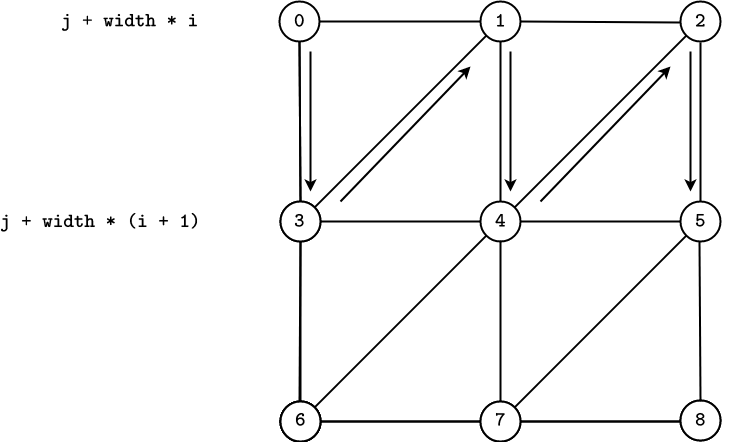
\includegraphics[width=0.9\textwidth]{atlod-naive-triangles}
  \caption{Example of a terrain layout for triangle strips. The looping index \texttt{i} goes from 0 to the terrain height and \texttt{j} from 0 to the terrain width. The final indices to be rendered are 0, 3, 1, 4, 2, 5, \texttt{RESTART}, 3, 6, 4, 7, 5, 8, \texttt{RESTART}.}\label{fig:naive-triangles}
\end{figure}

\subsubsection{Loading}
The method \texttt{loadBuffers()} is responsible for loading the data into the vertex and index buffer.
The first step is the generation of the normal vectors. This is done in the method \texttt{loadNormals()},
where the normals of each vertex are calculated into an intermediate vector \texttt{\_normals}.

The normals of the vertices are calculated by summing up the normal vectors 
of the four adjacent faces, which are given by calculating the cross product 
of the adjacent edges. The adjacent edges are given by subtracting 
neighboring vertices, as shown in figure \ref{fig:cross}.

\begin{figure}[H]
  \centering
  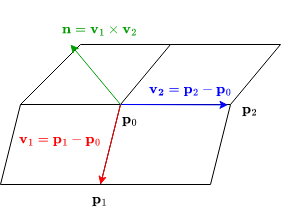
\includegraphics[width=0.6\textwidth]{cross-product}
  \caption{Example of a normal vector calculation of the bottom right face. The same process gets repeated for the other three adjacent faces.}\label{fig:cross}
\end{figure}

Afterwards the generation of the normal vectors, the vertices get 
generated and loaded onto the vertex buffer. The same happens for the indices.
After the data is loaded onto the GPU, the intermediate 
vectors \texttt{\_normals}, \texttt{\_vertices} and \texttt{\_indices} are cleared so that no unnecessary memory waste occurs.

\subsection{Rendering}
\subsubsection{Draw Call}
The entire terrain gets rendered using 1 draw call,
thanks to the index organisation with triangle strips 
and primitive restarting. Listing 

\subsubsection{Vertex Shader}
The vertex shader simply applies the model, view and projection 
matrices to the current position attribute, which is set as 
the fragment position output variable.
The texture coordinate output variable is set to 
the vertex attribute.

The normal vectors require a small additional operation before being sent to the fragment shader:
in order to allow for lighting with non-uniform scaling with the model matrix,
the \textit{normal matrix} must be applied to the normal vectors first \cite{learnopengl}.
The normal matrix is computed \textit{before} being set as a uniform variable, as follows:
$\mathbf{N} = (\mathbf{M}^{-1})^\top$.
Afterwards, it is converted to a $3 \times 3$ matrix in the vertex shader
and multiplied with the normal vector, which is then set as the normal output variable.

\subsubsection{Fragment Shader}
In the fragment shader, the lighting is computed with Phong shading 
and the overlay texture is applied (if one is used).
The lighting consists of an ambient light with a strength factor 0.5 and 
of a diffuse light. Both lights have a white color. 

The fog calculation is based on \cite{fogcalc} and can be adjusted with the argument \texttt{density}.
Listing \ref{lst:fogcalc} shows the function which calculates the fog factor and its usage:
\begin{lstlisting}[
  language={C++},
  label={lst:fogcalc},
  caption={The fog calculation in the fragment shader.}]
float calculateFog(float density) {
  float dist = length(cameraPos - FragPosition);
  float fogFactor = exp(-density * dist);
  return clamp(fogFactor, 0.0f, 1.0f);
}

void main() {
  // ...
  float fogFactor = calculateFog(fogDensity);
  color = mix(fogColour, color, fogFactor);
  // ...
  FragColor = vec4(color, 1.0f);
}
\end{lstlisting}


\section{GeoMipMapping}
This implementation of GeoMipMapping supports most basic functionalities described in the original paper, but differs in a few key aspects:
it draws some inspiration from other approaches, most notably from GPU-based Geometry Clipmaps \cite{gpugeomclipmaps} and certain minor elements from ``Terrain Rendering in Frostbite Using Procedural Shader Splatting'' \cite{procsplattingdice}.

Both approaches utilize a single flat mesh (positioned around the viewer in \cite{gpugeomclipmaps}, in world-space \cite{procsplattingdice}) and store the heightmap as a texture object. The height values are sampled in the vertex shader, which are then 
used to displace the flat mesh on the $y$-axis. 

The idea of using a texture image for the heightmap is applied to ATLOD's GeoMipMapping implementation.
Rather than generating vertex buffers for each block and loading in the height values into the vertices directly (as in the naive renderer implementation),
a single flat mesh with the side length of the block size is generated once at load time. At render time, for each block, the mesh is translated 
to the block's world-space position and the height values get sampled from the heightmap stored on the GPU.
The upcoming subsections describe the approach in greater detail.

\subsection{Class Structure}
GeoMipMapping contains the following members:
\begin{itemize}
  \item \texttt{unsigned \_blockSize}: the size of a single block.
  \item \texttt{unsigned \_nBlocksX, \_nBlocksZ}: the number of blocks in the $x$ and $z$-direction. 
        These two values are calculated in the constructor by dividing the terrain width and height by the block size and rounding the values down.
  \item \texttt{std::vector<GeoMipMappingBlock> \_blocks}: stores the blocks.
  \item \texttt{std::vector<unsigned> \_borderSizes, \_borderStarts, \_centerSizes, \_centerStarts}:
        Stores the start indices and sizes of the subsets of the index buffer containing the border areas and center areas (explained in more detail subsection ``Vertex and Index Organisation'').
  \item \texttt{unsigned \_vao, \_vbo, \_ebo}: the vertex array object, vertex buffer object and element buffer object respectively.
  \item \texttt{float \_baseDistance}: the distance until the next lower LOD level is chosen (explained in more detail in subsection ``LOD Selection'').
  \item \texttt{unsigned \_minLod, \_maxLod, \_maxPossibleLod}: the minimum and maximum user set LOD level, and the maximum possible LOD level.
\end{itemize}

\subsection{Blocks}
As previously described in the high-level overview of the GeoMipMapping algorithm, 
the algorithm splits up the terrain into square blocks of side length $2^n+1$.

In this implementation, a block is simply a structure containing information for a
particular section of the terrain. The struct \texttt{GeoMipMappingBlock}
represents such a block and contains the following fields:
\begin{itemize}
  \item \texttt{unsigned blockId}: the ID of the current block.
  \item \texttt{unsigned currentBorderBitmap}: the current border permutation as a bitmap.
  \item \texttt{glm::vec2 translation}: the 2-dimensional translation vector for translating the flat mesh to the block's actual world-space position.
  \item \texttt{glm::vec3 worldCenter}: the actual center position of that block in world-space, i.e. its $y$-coordinate is computed from the heightmap. 
        This field is used for the distance calculation for the LOD determination during rendering.
  \item \texttt{glm::vec3 p1, p2}: the two points defining the AABB of the block (corresponding to $\mathbf{p}_1$ and $\mathbf{p}_2$ in the subsection ``View-frustum Culling'' in ``Basics of Terrain Rendering'').
\end{itemize}

\subsection{Vertex and Index Organisation}
ATLOD's GeoMipMapping implementation consists of a single vertex buffer and index buffer.
The vertex buffer contains the vertices for a single flat $blockSize \times blockSize$ mesh centered around $(0,0,0)$, where $blockSize = 2^n + 1$ and $n$ is the maximum LOD level.
The vertices of the flat mesh only consist of 4-byte floating point $(x,z)$-coordinates, since the mesh is flat.

The index buffer contains the 4-byte unsigned integer indices of the flat mesh and is organized as follows:
the flat mesh is split up into its border area and center area.
The reason for splitting the mesh up this way will be made clear shortly.
The first part of the index buffer stores the indices of the border area
for every LOD level and border permutation, and
the second part of the index buffer stores the center area for every LOD level. 
What a \textit{border permutation} is will be explained in the next section.
Figure \ref{fig:atlod-geomipmapping-index-buffers} shows the described index buffer 
organisation.

\begin{figure}[H]
  \centering
  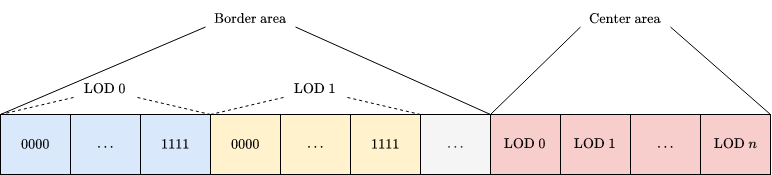
\includegraphics[width=1.0\textwidth]{atlod-geomipmapping-index-buffer.png}
  \caption{The index buffer organisation of the single flat block. The variable $n$ corresponds to the maximum LOD level.}\label{fig:atlod-geomipmapping-index-buffers}
\end{figure}

\subsubsection{Border Permutations}
A border permutation is defined to be a 4-tuple $(t,b,l,r)$,
where $t,b,l,r$ correspond to top, bottom, left and right, and where each entry is set to 1 if the block on 
the corresponding side has a lower LOD, and 0 otherwise. For example, if the top and right neighboring blocks
have a lower LOD than the current block, the border permutation is $(1,0,0,1)$.
These border permutations can also be expressed as bitfields, e.g. \texttt{1001},
which allows for easy indexing into the subset of the index buffer containing the relevant indices.
The number of possible permutations is $2^4=16$.
In order for this approach to work, the difference in LOD level between any two bordering blocks 
must be at most 1. 
Figure \ref{fig:atlod-geomipmapping-crack-avoidance} shows all possible border permutations of a $5 \times 5$ block at LOD level 2.

\begin{figure}[H]
  \centering
  \subfloat[\centering \texttt{0000}.]{{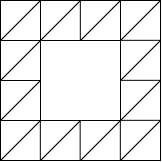
\includegraphics[width=0.17\textwidth]{atlod-geomipmapping-0000.png} }}
  \qquad
  \subfloat[\centering \texttt{0001}.]{{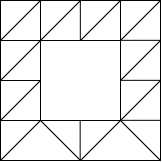
\includegraphics[width=0.17\textwidth]{atlod-geomipmapping-0001.png} }}
  \qquad
  \subfloat[\centering \texttt{0010}.]{{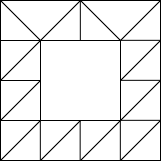
\includegraphics[width=0.17\textwidth]{atlod-geomipmapping-0010.png} }}
  \qquad
  \subfloat[\centering \texttt{0011}.]{{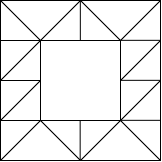
\includegraphics[width=0.17\textwidth]{atlod-geomipmapping-0011.png} }}

  \subfloat[\centering \texttt{0100}.]{{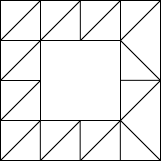
\includegraphics[width=0.17\textwidth]{atlod-geomipmapping-0100.png} }}
  \qquad
  \subfloat[\centering \texttt{0101}.]{{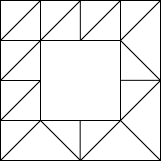
\includegraphics[width=0.17\textwidth]{atlod-geomipmapping-0101.png} }}
  \qquad
  \subfloat[\centering \texttt{0110}.]{{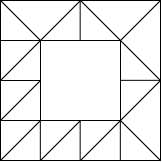
\includegraphics[width=0.17\textwidth]{atlod-geomipmapping-0110.png} }}
  \qquad
  \subfloat[\centering \texttt{0111}.]{{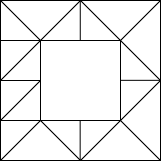
\includegraphics[width=0.17\textwidth]{atlod-geomipmapping-0111.png} }}

  \subfloat[\centering \texttt{1000}.]{{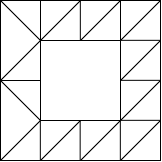
\includegraphics[width=0.17\textwidth]{atlod-geomipmapping-1000.png} }}
  \qquad
  \subfloat[\centering \texttt{1001}.]{{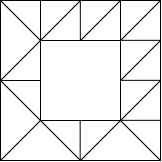
\includegraphics[width=0.17\textwidth]{atlod-geomipmapping-1001.png} }}
  \qquad
  \subfloat[\centering \texttt{1010}.]{{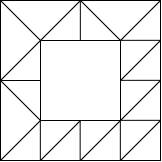
\includegraphics[width=0.17\textwidth]{atlod-geomipmapping-1010.png} }}
  \qquad
  \subfloat[\centering \texttt{1011}.]{{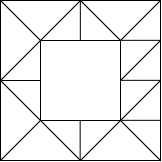
\includegraphics[width=0.17\textwidth]{atlod-geomipmapping-1011.png} }}

  \subfloat[\centering \texttt{1100}.]{{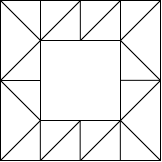
\includegraphics[width=0.17\textwidth]{atlod-geomipmapping-1100.png} }}
  \qquad
  \subfloat[\centering \texttt{1101}.]{{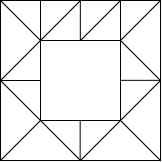
\includegraphics[width=0.17\textwidth]{atlod-geomipmapping-1101.png} }}
  \qquad
  \subfloat[\centering \texttt{1110}.]{{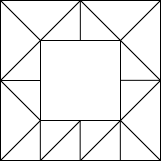
\includegraphics[width=0.17\textwidth]{atlod-geomipmapping-1110.png} }}
  \qquad
  \subfloat[\centering \texttt{1111}.]{{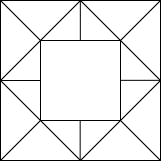
\includegraphics[width=0.17\textwidth]{atlod-geomipmapping-1111.png} }}
  \caption{Every possible border permutation for a LOD 2 GeoMipMap of a $5 \times 5$ block. The center subblocks have been omitted from the illustration.}\label{fig:atlod-geomipmapping-crack-avoidance}
\end{figure}

This makes clear why the flat mesh is split into its border and center area.
The center area only depends on the LOD level and is the same 
regardless of the current border permutation. 
Not splitting the flat mesh up into its border and center area 
would require longer index buffer generation times and consume 
significantly more GPU memory.

\subsubsection{Starts and Sizes Lists}
The organisation of the index buffer as presented requires some additional
management of the start indices and sizes of the subsets of the index buffer. As previously mentioned, the \texttt{GeoMipMapping} class 
contains four members of the type \texttt{std::vector<unsigned>}:
\texttt{\_borderStarts}, \texttt{\_borderSizes}, \texttt{\_centerStarts} and \texttt{\_centerSizes}.
The \texttt{\_borderStarts} and \texttt{\_borderSizes} lists store the starting index 
(into the index buffer) and 
the number of indices, for a subset of the index buffer containing the indices of the border area for a given border permutation and LOD level.
Both the lists are indexed by multiplying the current LOD level by 16 
and then adding the current border permutation to it.
The \texttt{\_centerStarts} and \texttt{\_centerSizes} lists are indexed similarly,
except that they are indexed simply with the current LOD level.

In order to illustrate the idea more clearly, the following example is given:
say that the current block has a LOD level of 1 and every neighboring block has the 
same LOD level (i.e. the border permutation is $(0,0,0,0)$). 
We want to render the block, which means 
we need to retrieve the indices for the flat mesh 
at the LOD level 1 and for the border permutation \texttt{0000}.
The start index and the size for the border area are retrieved with \texttt{\_borderStarts[1 * 16 + 0b0000]}
and \texttt{\_borderSizes[1 * 16 + 0b0000]} respectively, and for 
the center area with \texttt{\_centerStarts[1]} and \texttt{\_centerSizes[1]}.
These four values are passed to the two \texttt{glDrawElements()} draw calls for the block,
which renders the flat mesh at the chosen LOD level 1 and border permutation $(0,0,0,0)$.
The full rendering process is described in the subsection ``Rendering'' of this section.
Figure \ref{fig:atlod-starts-sizes-example} illustrates this example.

\begin{figure}[H]
  \centering
  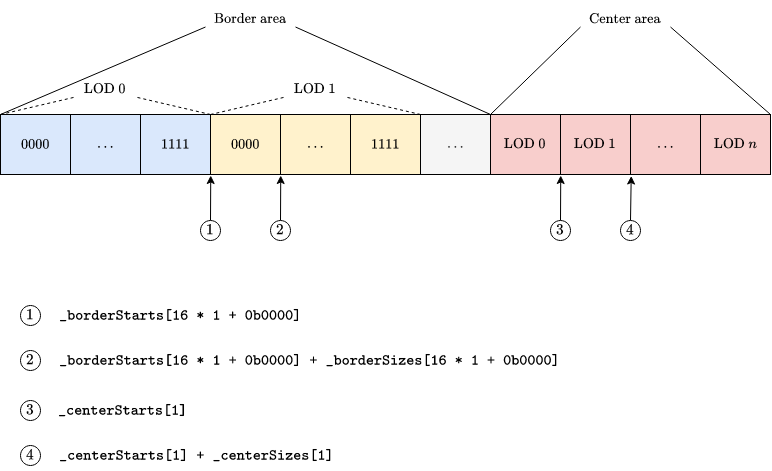
\includegraphics[width=1.0\textwidth]{atlod-starts-sizes-example.png}
  \caption{Illustration of accessing the start index and size of the subsets of the index buffer for LOD 1 and border permutation $(0,0,0,0)$}\label{fig:atlod-starts-sizes-example}
\end{figure}

\subsubsection{Loading}
Now that the organisation of the vertices and indices 
has been presented, the loading mechanisms are described.
The vertex and index buffers get loaded in the method \texttt{loadBuffers()},
which calls the two helper methods \texttt{loadVertices()} an \texttt{loadIndices()}.

The method \texttt{loadVertices()} (listing \ref{lst:loadverts}) simply generates the vertex array object with its ID stored in the field \texttt{\_vao}
and loads the vertices of the flat mesh of size $blockSize \times blockSize$
centered around $(0,0,0)$ into a vertex buffer with its ID stored in the field \texttt{\_vbo}.
\begin{lstlisting}[
  language=C++,
  label={lst:loadverts},
  caption={Method \texttt{GeoMipMapping::loadVertices()} that generates the vertex array object and loads the
  vertex buffer with the flat mesh of size $blockSize \times blockSize$ centered around $(0,0,0)$.}]
void GeoMipMapping::loadVertices()
{
    for (int i = 0; i < _blockSize; i++) {
        for (int j = 0; j < _blockSize; j++) {
            // Load vertices around center point 
            float x = (-(float)_blockSize / 2.0f + (float)_blockSize * j / (float)_blockSize);
            float z = (-(float)_blockSize / 2.0f + (float)_blockSize * i / (float)_blockSize);

            _vertices.push_back(x); // Position x 
            _vertices.push_back(z); // Position z 
        }
    }

    glGenVertexArrays(1, &_vao);
    glBindVertexArray(_vao);

    glGenBuffers(1, &_vbo);
    glBindBuffer(GL_ARRAY_BUFFER, _vbo);
    glBufferData(GL_ARRAY_BUFFER, _vertices.size() * sizeof(float), &_vertices[0], GL_STATIC_DRAW);

    // Position attribute
    glVertexAttribPointer(0, 2, GL_FLOAT, GL_FALSE, 2 * sizeof(float), (void*)0);
    glEnableVertexAttribArray(0);
}
\end{lstlisting}

The index loading mechanism is significantly more complex.
The top-level index loading method \texttt{loadIndices()}
performs the following operations:
\begin{itemize}
  \item It loads the LOD 0 and LOD 1 representation of the flat mesh using \texttt{loadLod0()} and \texttt{loadLod1()} respectively. The LOD 0 and LOD 1 indices require special treatment. They are stored only as borders and do not have a center.
        If \texttt{\_minLod} is greater than 1, then this step is skipped.
  \item It loads the rest of the indices from the \texttt{\_minLod} to \texttt{\_maxLod}, by first loading in the border indices with \texttt{loadBorderAreaForLod()}
        and then the center areas with \texttt{loadCenterAreaForLod()}.
\end{itemize}

The \texttt{loadBorderAreaForLod()} method accepts the LOD level to be loaded \texttt{lod} and first iterates from 0 to 16 
(i.e. for every possible border permutation) and calls \texttt{loadBorderAreaForPermutation(lod, i)}.
The function \texttt{loadBorderAreaForPermutation()} takes the LOD level to be loaded and the 
border permutation to be loaded and calls the following 8 helper methods:
\begin{itemize}
  \item \texttt{loadTopLeftCorner(step, permutation)}
  \item \texttt{loadTopBorder(step, permutation)}
  \item \texttt{loadTopRightCorner(step, permutation)}
  \item \texttt{loadRightBorder(step, permutation)}
  \item \texttt{loadBottomRightCorner(step, permutation)}
  \item \texttt{loadBottomBorder(step, permutation)}
  \item \texttt{loadBottomLeftCorner(step, permutation)}
  \item \texttt{loadLeftBorder(step, permutation)}
\end{itemize}

Each of the eight method calls loads in the corresponding side or corner 
at the LOD level given by \texttt{step} and for the border permutation
given by \texttt{permutation}. The variable \texttt{step} 
is the step size (i.e. how many vertices to skip due to the LOD when computing the mesh)
and is computed directly from \texttt{lod} with \texttt{step = std::pow(2, \_maxLod - lod)}.

Listing \ref{lst:loadtopleftcorner} shows the method \texttt{loadTopLeftCorner()}.
The other methods work similarly.

\begin{lstlisting}[
  language=C++,
  label={lst:loadtopleftcorner},
  caption={Method \texttt{GeoMipMapping::loadTopLeftCorner()} which loads in the indices of the top left corner of the flat mesh for a given LOD level and border permutation}]
unsigned GeoMipMapping::loadTopLeftCorner(unsigned step, unsigned permutation)
{
    unsigned count = 0;
    if ((permutation & LEFT_BORDER_BITMASK) && (permutation & TOP_BORDER_BITMASK)) { /* bitmask is 1_1_ */
        /*
          * *- - -*- - -*
          * |\         /|
          * |  \     /  |
          * |    \ /    |
          * *     *- - -*
          * |    /|
          * |  /  |
          * |/    |
          * *- - -*
          *
          */

        pushIndex(2 * step, step);
        pushIndex(2 * step, 0);
        pushIndex(step, step);
        pushIndex(0, 0);
        pushIndex(0, 2 * step);
        indices.push_back(RESTART_INDEX);

        pushIndex(step, 2 * step);
        pushIndex(step, step);
        pushIndex(0, 2 * step);
        indices.push_back(RESTART_INDEX);

        count += 10;

    } else if (permutation & LEFT_BORDER_BITMASK) { /* bitmask is 1_0_*/

        /*
          * *- - -*- - -*
          * |\    |    /|
          * |  \  |  /  |
          * |    \|/    |
          * *     *- - -*
          * |    /|
          * |  /  |
          * |/    |
          * *- - -*
          *
          */

        pushIndex(step, 0);
        pushIndex(0, 0);
        pushIndex(step, step);
        pushIndex(0, 2 * step);
        pushIndex(step, 2 * step);
        indices.push_back(RESTART_INDEX);

        pushIndex(step, 0);
        pushIndex(step, step);
        pushIndex(2 * step, 0);
        pushIndex(2 * step, step);
        indices.push_back(RESTART_INDEX);

        count += 11;

    } else if (permutation & TOP_BORDER_BITMASK) { /* bitmask is 0_1_ */
        /*
          * *- - -*- - -*
          * |\         /|
          * |  \     /  |
          * |    \ /    |
          * *- - -*- - -*
          * |    /|
          * |  /  |
          * |/    |
          * *- - -*
          *
          */

        pushIndex(0, step);
        pushIndex(0, 2 * step);
        pushIndex(step, step);
        pushIndex(step, 2 * step);
        indices.push_back(RESTART_INDEX);

        pushIndex(2 * step, step);
        pushIndex(2 * step, 0);
        pushIndex(step, step);
        pushIndex(0, 0);
        pushIndex(0, step);
        indices.push_back(RESTART_INDEX);

        count += 11;

    } else { /* bitmask is 0_0_*/
        /*
          * *- - -*- - -*
          * |    /|    /|
          * |  /  |  /  |
          * |/    |/    |
          * *- - -*- - -*
          * |    /|
          * |  /  |
          * |/    |
          * *- - -*
          *
          */

        pushIndex(0, step);
        pushIndex(0, 2 * step);
        pushIndex(step, step);
        pushIndex(step, 2 * step);
        indices.push_back(RESTART_INDEX);

        pushIndex(0, 0);
        pushIndex(0, step);
        pushIndex(step, 0);
        pushIndex(step, step);
        pushIndex(2 * step, 0);
        pushIndex(2 * step, step);
        indices.push_back(RESTART_INDEX);

        count += 12;
    }

    return count;
}
\end{lstlisting}

The \texttt{loadCenterAreaForLod()} method accepts the LOD level to be loaded \texttt{lod} as well and 
simply loads the indices with the given LOD resolution into \texttt{\_indices}, similarly to 
the index loading of the naive brute-force algorithm. 

After loading the indices and the vertices, 
the intermediate vectors \texttt{\_vertices} and \texttt{\_indices} get cleared.

\subsection{Rendering}
The method \texttt{render()} that is called each frame performs in two phases:
\begin{itemize}
  \item The first phase iterates through every block and updates the LOD level of the block (described in the next subsection ``LOD Selection'')
        and then updates the border permutation bitmap.
  \item The second phase iterates through every block again and performs view-frustum culling, sets the uniform variables in the shader,
        and finally renders the the border area and center area of that block.
\end{itemize}

\subsubsection{LOD Selection}
The LOD of ATLOD's GeoMipMapping implementation is based on the Euclidean distance $dist$ between 
the camera's position $\mathbf{p}_{camPos}$ 
and the block's center point $\mathbf{p}_{blockCenter}$
\begin{align*}
  dist = \sqrt{ \begin{aligned} & (blockCenter_x - camPos_x)^2 + (blockCenter_y - camPos_y)^2 \\
          & + (blockCenter_z-camPos_z)^2 \end{aligned}}.
\end{align*}
A minor optimization for this calculation is possible by instead calculating the LOD using the squared distance, 
which avoids an expensive square-root call.

Two different LOD determination modes are possible: the \textit{linearly growing distance} and the \textit{exponentially growing distance}.
Both use a base distance value $baseDist$ which 
can be set by the user. Note that $baseDist$ should be larger than $blockSize$,
as otherwise cracks in the terrain may occur, but also not too large, 
so that the performance is still adequate.
The LOD computed by the linearly growing distance can be defined with the following recursive formula
\begin{align*}
  lod_{lin}(dist, i) = 
  \begin{cases}
    l - i  + 1& dist \leq i \cdot baseDist\\
    lod_{lin}(dist, i + 1) & i \cdot baseDist < dist < (l + 1) \cdot baseDist\\
    0 & \text{otherwise}
  \end{cases},
\end{align*}
where $i$ starts at 1 and $l$ is the maximum LOD level.
As a basic example, say that $l=3,baseDist=100,dist=250$.
We begin computing the LOD level with $lod_{lin}(250,1)$.
The second condition $1 \cdot 100 < 250 < 4 \cdot 100$ holds, so we continue with $lod_{lin}(250,2)$.
Again, the second condition $2 \cdot 100 < 250 < 4 \cdot 100$ holds, so we continue with $lod_{lin}(250,3)$.
Now, the first condition $250 \leq 3 \cdot 100$ holds, so the entire expression evaluates to $3-3+1=1$,
which means we set the LOD level of the block to 1.

The exponentially growing distance is defined very similarly:
\begin{align*}
  lod_{exp}(dist, i) = 
  \begin{cases}
    l - i + 1 & dist \leq i \cdot baseDist\\
    lod_{exp}(dist, 2i) & i \cdot baseDist < dist < (l+1) \cdot baseDist\\
    0 & \text{otherwise}
  \end{cases}.
\end{align*}

The above expressions are implemented in the \texttt{GeoMipMapping} class in a single method \texttt{determineLodDistance()}.
The LOD determination mode can be set with the boolean argument \texttt{doubleEachLevel}.
Additionally, the minimum and maximum LOD levels can be manually set to be different from 0 and $l$ respectively 
by the user, with the fields \texttt{\_minLod} and \texttt{\_maxLod}. 
Note that the user defined \texttt{\_minLod} and \texttt{\_maxLod} values
are both set to $\max\{0,\texttt{\_minLod}\}$ and $\min\{l,\texttt{\_maxLod}\}$ respectively in the constructor, 
so that the LOD level does not go out of bounds.
Listing \ref{lst:determineloddistance} shows the method \texttt{determineLodDistance}.

\begin{lstlisting}[
  language={C++},
  label={lst:determineloddistance},
  caption={Method \texttt{GeoMipMapping::determineLodDistance()} that determines the LOD level of a block 
  based on its distance to the camera.}]
unsigned GeoMipMapping::determineLodDistance(float squareDistance, float baseDist, bool doubleEachLevel)
{
    unsigned distancePower = 1;
    for (unsigned i = 0; i < _maxLod - _minLod; i++) {
        if (squaredDistance < distancePower * distancePower * baseDist * baseDist)
            return _maxLod - i;

        if (doubleEachLevel)
            distancePower <<= 1;
        else
            distancePower++;
    }
    return _minLod;
}
\end{lstlisting}

Figure \ref{fig:atlod-lin-exp} shows both LOD determination modes in action.
\begin{figure}[H]
  \centering
  \subfloat[\centering Linearly growing distance mode.]{{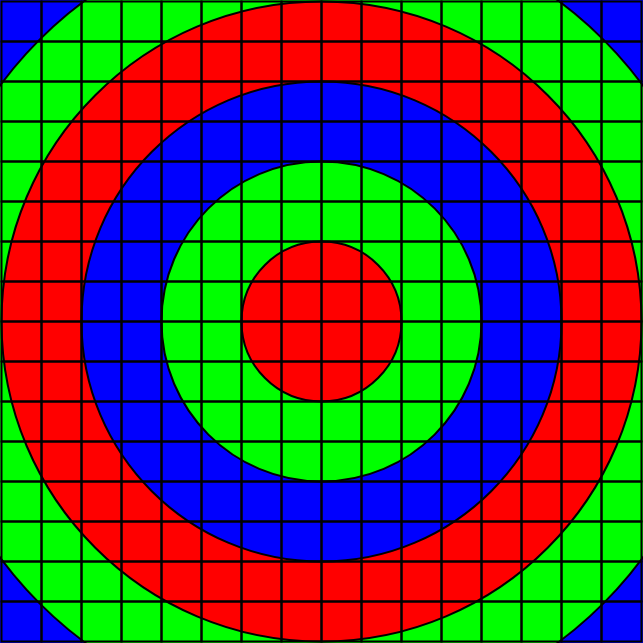
\includegraphics[width=0.4\textwidth]{atlod-lod-linear} }}
  \qquad
  \subfloat[\centering Exponentially growing distance mode.]{{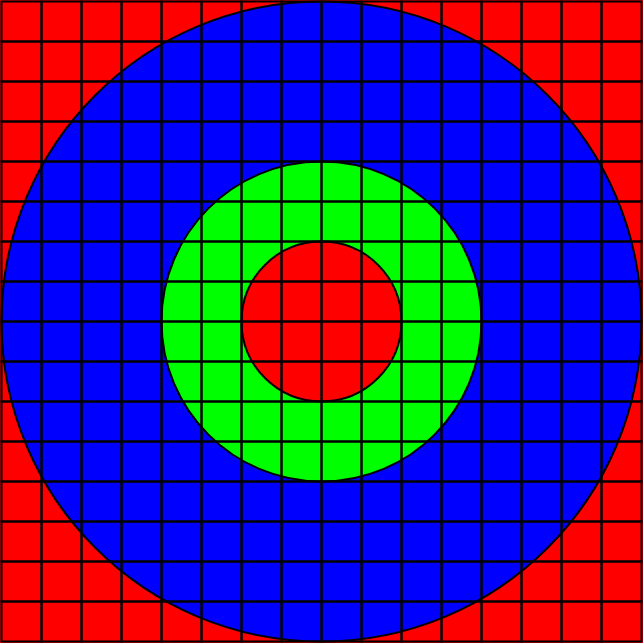
\includegraphics[width=0.4\textwidth]{atlod-lod-exponential} }}%
  \caption{Illustration of a flat terrain showcasing the linearly growing distance mode (a) and exponentially growing distance mode (b). The red, green and blue colors indicate successively lower LOD levels, starting from the maximum level in the center.}\label{fig:atlod-lin-exp}
\end{figure}

\subsubsection{Border Bitmap Calculation}
Listing \ref{lst:borderbitmap} shows the calculation of the border permutation bitmap for a given block.
The first step consists of calculating the minimum and maximum $x$ and $z$ block indices
in order to avoid going out of bounds. Afterwards, the LOD of the four neighboring blocks
gets retrieved and the bitmap is set depending on whether the corresponding side 
has a lower LOD or not, as described previously.
\begin{lstlisting}[
  language={C++},
  label={lst:borderbitmap},
  caption={The method \texttt{GeoMipMapping::calculateBorderBitmap()} which computes the border permutation bitmap for a given block.}]
unsigned GeoMipMapping::calculateBorderBitmap(unsigned currentBlockId, unsigned x, unsigned z)
{
    unsigned currentLod = _blocks[currentBlockId].currentLod;

    unsigned maxX = std::max((int)x - 1, 0);
    unsigned minX = std::min((int)x + 1, (int)_nBlocksX - 1);
    unsigned maxZ = std::max((int)z - 1, 0);
    unsigned minZ = std::min((int)z + 1, (int)_nBlocksZ - 1);

    GeoMipMappingBlock& leftBlock = getBlock(maxX, z);
    GeoMipMappingBlock& rightBlock = getBlock(minX, z);
    GeoMipMappingBlock& topBlock = getBlock(x, maxZ);
    GeoMipMappingBlock& bottomBlock = getBlock(x, minZ);

    unsigned leftLower = currentLod > leftBlock.currentLod ? 1 : 0;
    unsigned rightLower = currentLod > rightBlock.currentLod ? 1 : 0;
    unsigned topLower = currentLod > topBlock.currentLod ? 1 : 0;
    unsigned bottomLower = currentLod > bottomBlock.currentLod ? 1 : 0;

    return (leftLower << 3) | (rightLower << 2) | (topLower << 1) | bottomLower;
}
\end{lstlisting}


\subsubsection{Draw Calls} 
Two draw calls are performed per block: one for the center area and one for the border area.
The arguments of the draw calls follow the logic described in ``Vertex and Index Organisation''.
Listing \ref{lst:drawcalls} shows the two draw calls which occur inside the second phase of the \texttt{render()} method.

\begin{lstlisting}[
  language={C++},
  label={lst:drawcalls},
  caption={The two draw calls occuring inside the second loop over all blocks inside the method \texttt{GeoMipMapping::render().}}]
unsigned currentIndex = block.currentLod - _minLod;

// First render the center subblocks (only for LOD >= 2, since
// LOD 0 and 1 do not have a center block) */
if (block._currentLod >= 2) {
    glDrawElements(GL_TRIANGLE_STRIP,
        centerSizes[currentIndex],
        GL_UNSIGNED_INT,
        (void*)(centerStarts[currentIndex] * sizeof(unsigned)));
}

// Then render the border subblocks
currentIndex = currentIndex * 16 + block._currentBorderBitmap;
glDrawElements(GL_TRIANGLE_STRIP,
    borderSizes[currentIndex],
    GL_UNSIGNED_INT,
    (void*)(borderStarts[currentIndex] * sizeof(unsigned)));
\end{lstlisting}

\subsubsection{Vertex Shader}
The vertex shader calculates the heightmap texture coordinate 
using the vertex position attribute, the texture width and height given as uniforms, 
and the block's translation vector given as an uniform.

Afterwards, it samples the height from the heightmap texture 
and multiplies it by 65535 (since the texture image is normalized with all values from 0 to 1).

Next, it translates the vertex from its initial position around $(0,0,0)$ to its actual world-space 
position using the translation vector and the $y$-coordinate is set to the sampled height.
Listing \ref{lst:vertexshader} shows the source code of the vertex shader.

\begin{lstlisting}[
  language={C++},
  label={lst:vertexshader},
  caption={The vertex shader of the GeoMipMapping implementation.}]
#version 330 core
layout (location = 0) in vec2 aPos;

out vec3 FragPosition;

uniform mat4 projection;
uniform mat4 view;
uniform mat4 model;
uniform vec2 offset;
uniform sampler2D heightmapTexture;
uniform float textureWidth;
uniform float textureHeight;

void main()
{
    vec2 texPos =  vec2((aPos.x + offset.x + 0.5 * textureWidth) / (textureWidth),
                        (aPos.y + offset.y + 0.5 * textureHeight) / (textureHeight));

    float height = texture(heightmapTexture, texPos).r;
    float y = height * 65535;

    vec3 actualPos = vec3(aPos.x + offset.x, y, aPos.y + offset.y);

    FragPosition = vec3(model * vec4(actualPos, 1.0));
    gl_Position = projection * view * model * vec4(actualPos, 1.0);
}
\end{lstlisting}

\subsubsection{Fragment Shader}
The fragment shader shades the fragment using the Phong shading method
and is exactly the same as the naive brute-force algorithm in terms of computing the lighting. The main 
difference is the way how normals are handled. 
Recall that the vertices contained no normal vector attribute.
The normal vectors are instead calculated based on the method described in \cite{procsplattingdice}:
first, the heightmap is sampled at the four orthogonally neighboring points for the height values $y_{left}, y_{right}, y_{top}, y_{bottom}$.
Using these four values, the slope in $x$ and $z$-direction can be calculated by computing
\begin{align*}
  dx = y_{left} - y_{right}\\
  dz = y_{top} - y_{bottom}.
\end{align*}
These values can now be used to create a normal vector
\begin{align*}
  \mathbf{n} = \frac{(dx, 2, dz)}{\lVert (dx, 2, dz) \rVert}.
\end{align*}
Afterwards, this normal vector can be used as usual to compute diffuse lighting.
Listing \ref{lst:normalcalc} shows the calculation of the normal vector from the heightmap texture.

\begin{lstlisting}[
  language={C++},
  label={lst:normalcalc},
  caption={Calculating the normal vector in the fragment shader using the heightmap texture.}]
vec2 texPos = vec2((FragPosition.x + 0.5 * textureWidth) / textureWidth, (FragPosition.z + 0.5 * textureHeight) / textureHeight);

float leftHeight = texture(heightmapTexture, texPos - vec2(1.0 / textureWidth, 0)).r;
float rightHeight = texture(heightmapTexture, texPos + vec2(1.0 / textureWidth, 0)).r;
float upHeight = texture(heightmapTexture, texPos + vec2(0, 1.0 / textureHeight)).r;
float downHeight = texture(heightmapTexture, texPos - vec2(0, 1.0 / textureHeight)).r;

// Multiply with 65535 to denormalize
float dx = (leftHeight - rightHeight) * yScale * 65535;
float dz = (downHeight - upHeight) * yScale * 65535;

vec3 normal = normalize(vec3(dx, 2.0f, dz));

// Continue with diffuse lighting ...
\end{lstlisting}

The fog calculation is exactly the same as in the naive brute-force rendering algorithm (listing \ref{lst:fogcalc}).
